\documentclass[conference]{IEEEtran}
% \IEEEoverridecommandlockouts
% The preceding line is only needed to identify funding in the first footnote. If that is unneeded, please comment it out.
\usepackage{cite}
\usepackage{amsmath,amssymb,amsfonts}
\usepackage{graphicx}
\usepackage{textcomp}
\usepackage{algorithm}
\usepackage{algpseudocode}
\usepackage{tabularx,booktabs}
\usepackage{xcolor}
\def\BibTeX{{\rm B\kern-.05em{\sc i\kern-.025em b}\kern-.08em
    T\kern-.1667em\lower.7ex\hbox{E}\kern-.125emX}}
\begin{document}

% \title{Multiple Channel Perfect Reconstruction trans-multiplexer using Wavelet transform Techniques for Satellite Communications}
\title{Wavelet-based Perfect Reconstruction Trans-multiplexer for Satellite Communications}

\makeatletter
\newcommand{\linebreakand}{%
  \end{@IEEEauthorhalign}
  \hfill\mbox{}\par
  \mbox{}\hfill\begin{@IEEEauthorhalign}
}

\makeatother
\renewcommand\IEEEkeywordsname{Keywords}


\author{\IEEEauthorblockN{Kaustubh Venkatesh}
\IEEEauthorblockA{\textit{Department of Electronics}\\
\textit{and Telecommunication Engineering} \\
\textit{Sardar Patel Institute of Technology}\\
Mumbai-58, India \\
kaustubh.v@spit.ac.in}
\and
\IEEEauthorblockN{Gokul Nair}
\IEEEauthorblockA{\textit{Department of Electronics}\\
\textit{and Telecommunication Engineering} \\
\textit{Sardar Patel Institute of Technology}\\
Mumbai-58, India \\
gokul.nair@spit.ac.in}
\and
\IEEEauthorblockN{Arseta Singh}
\IEEEauthorblockA{\textit{Department of Electronics}\\
\textit{and Telecommunication Engineering} \\
\textit{Sardar Patel Institute of Technology}\\
Mumbai-58, India \\
arseta.singh@spit.ac.in}
\linebreakand
\IEEEauthorblockN{Dr. Sukanya Kulkarni}
\IEEEauthorblockA{\textit{Department of Electronics}\\
\textit{and Telecommunication Engineering} \\
\textit{Sardar Patel Institute of Technology}\\
Mumbai-58, India \\
sukanya\_kulkarni@spit.ac.in}
\and
\IEEEauthorblockN{Dr. Preetida Jani}
\IEEEauthorblockA{\textit{Department of}\\ \textit{Computer Engineering} \\
\textit{Sardar Patel Institute of Technology}\\
Mumbai-58, India \\
preeti.vinayakray@spit.ac.in}
}


\maketitle

\begin{abstract}
Satellite communication has become firmly established as one of three basic techniques for long-distance telecommunications. Multiplexing in satellite systems preserves channel resources and improves the temporal and computational complexity of the system. Filter bank-based multiplexing solutions are gaining popularity in the domain, as they achieve high data rates with relatively low error rates. Trans-multiplexers are applications of filter banks that convert time-division-multiplexed (TDM) signals to frequency-division-multiplexed (FDM) signals for transmission over a channel. Most trans-multiplexer systems use Fourier and Cosine transforms for filter design and signal reconstruction, which do not offer Perfect Reconstruction (PR) as the time domain information of the signal is discarded. This paper presents an algorithm that utilizes wavelet transform techniques for filter design to be used in trans-multiplexers. The work realizes the designed filters and trans-multiplexer system in MATLAB, and its performance is evaluated by testing with various channel models and mother wavelets. The simulated system outperforms a similar conventional system by a factor of $10^{-4}$.
\end{abstract}

\begin{IEEEkeywords}
Wavelet transform, Digital Filter Banks, trans-multiplexers, Satellite communications
\end{IEEEkeywords}

\section{Introduction}
Satellite systems play a major role in global communications, being used in television, telephone, radio, internet, and military applications. These systems transmit and receive various data types such as voice, video, geo-location, and TCP/IP packets. These systems are complex and need to be computationally efficient due to the availability of limited resources. Thus, communication systems in these satellites must be efficient and have low bit error rates. To better utilize scarce channel resources and to improve temporal and computational complexity, these systems use multiplexing to process multiple signals at the same time. Multiplexing sends multiple signals or streams of information over a communications link simultaneously in the form of a single, complex signal. Filter Bank based solutions have been gaining popularity as these can increase data rates while reducing error rates. \par

Trans-multiplexers are the application of digital filter banks that are used to convert time-division-multiplexed signals (TDM) to frequency-division-multiplexed (FDM) signals. In a trans-multiplexer, for TDM-FDM conversion, the input signal {x(n)} is a time-division-multiplexed signal consisting of $N$ signals. Each signal is then interpolated and modulated on a different carrier frequency to obtain an FDM signal for transmission. For FDM-TDM conversion, the composite signal is separated by filtering into $N$ components and decimating which results in TDM signals. Conventionally, trans-multiplexer systems utilize cosine and Fourier transformation functions for signal reconstruction and filter design. These however do not provide perfect reconstruction of the signals. \par

To solve the problem of cross-talk due to the loss of time-domain information, the use of wavelet transform has been proposed. This is because wavelets offer localization in the frequency domain i.e. high frequency resolution at low frequencies and high time resolution at high frequencies. In the Discrete Wavelet transform (DWT), the wavelets are discretely sampled, preserving both the frequency and location information of the signal. Moreover, the DWT algorithm has a time complexity of $O(N)$ instead of $O(N*log(N))$, thus making the system more efficient. The DWT of a signal is calculated by passing it through a series of filters.

\section{Related Work}

The use of filter banks as an alternative to conventional signal processing systems is a well-explored topic. The improved data rates, as well as error rates achieved by such systems, have been proven theoretically and practically. A sizeable number of studies explore the underlying theory and mathematics behind trans-multiplexers as an application of filter banks. \cite{b1}  introduces the research proposal and delineates the project deliverables. \cite{b2}, \cite{b3}, \cite{b5} explore wavelet transform technique to realise FIR filter banks but does not highlight a generalised algorithm.  \cite{b9} explores the concept of perfect trans-multiplexers, whereas \cite{b4}, \cite{mallat_paper}, and \cite{b16} explore the Wavelet Transform (WT). Various studies use conventional transformation functions such as Fourier and cosine \cite{b6} \cite{b10}, which result in some amount of amplitude distortion and cross-talk, which is undesirable in satellite systems. \cite{b7}, \cite{b8}, \cite{b14} and \cite{b13} explore the concept of perfect reconstruction (PR) and achieving a pure delay as the determinant of the co-factor matrix of the filter bank coefficients. Thus, subsequent studies have proposed the use of wavelet transform \cite{b2} \cite{b5} \cite{b11} as an alternative to improve system performance. \cite{b15} proposes a method to design PR trans-multiplexers for on-board satellite systems.


Thus, various studies have proposed algorithms for wavelet-based filter bank design, but do not consider the case of trans-multiplexers. Moreover, these studies merely describe the algorithm without proper implementation, simulation and testing. The main contribution of this study is the design of trans-multiplexer using wavelet based  filter banks. Hence, the proposed wavelet based algorithm is considered to overcome the limitations of existing systems. The work implements the specified filters and trans-multiplexer system in MATLAB, and its performance is assessed using a variety of channel models and mother wavelets. The organization of the paper is as follows. Section III delineates the process flow diagram and algorithm. Section IV defines the evaluation metrics and discusses the performance of the system.

\section{Methodology}
\subsection{Algorithm and Process Flow Model}
The design of wavelet transform based filters for a near perfect reconstruction (PR) trans-multiplexer can be be explained using the steps depicted in Algorithm \ref{alg:cap}. The algorithm is based on the theory discussed in \cite{b2} \cite{b5} \cite{b9}.

\begin{algorithm}
\caption{Algorithm for filter design}\label{alg:cap}
\begin{algorithmic}
\Require Should satisfy the Matrix Equation
\Ensure $H_i$ has Zeros at $z=-1$
\Ensure Degree of poylnomials = $(2N+1)$
\For{n = 0 to n = N}
\State Selection of generic Transmission polynomial $T_{i,j}(z)$
\State Factorization of $T_{i,j}$ into Synthesis filter $H_i(z)$ \& Analysis filter $G_j(z)$
\State Choose Synthesis and Analysis filters from the generated Co-factor Matrix
\State Determination of Impulse, Frequency and Phase responses of $H_i$ and $G_j$
\Ensure Determinant results in Pure Delay
\State Calculation of Aggregated Response of the System
\State Incorporation in designed system \& Evaluation of Performance
\EndFor
\end{algorithmic}
\end{algorithm}

% \begin{figure}[htpb]
% \centering
% 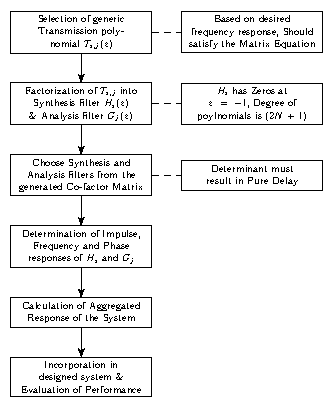
\includegraphics[width = 9cm]{Design_algorithm.pdf}
% \caption{Flow diagram of the algorithm.}
% \label{algo}
% \end{figure}

\subsection{Designed System}
The following system design was conducted based on given specifications for 3  input signals ($N = 3$). These include 2 voice signals in the band of 20 Hz - 4 kHz and 1 for metadata in the band of 300 Hz - 3.4 kHz. The same algorithm can be extended to include more number of signals in other frequency bands. The frequency factor $M$ was chosen as 4. Using the above algorithm, the response of the system for analysis and synthesis steps are shown in Fig. \ref{agg}. Fig. \ref{fig:block} shows the block diagram of the system.

\begin{figure}
    \centering
    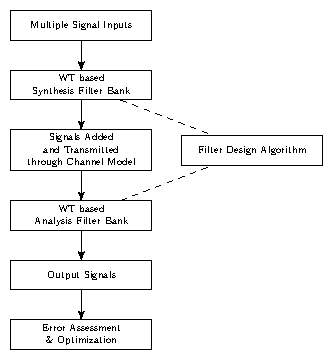
\includegraphics[width=8.75cm]{Block_diagram.pdf}
    \caption{Block diagram of the system.}
    \label{fig:block}
\end{figure}

% \begin{figure}[htpb]
% \centering
% 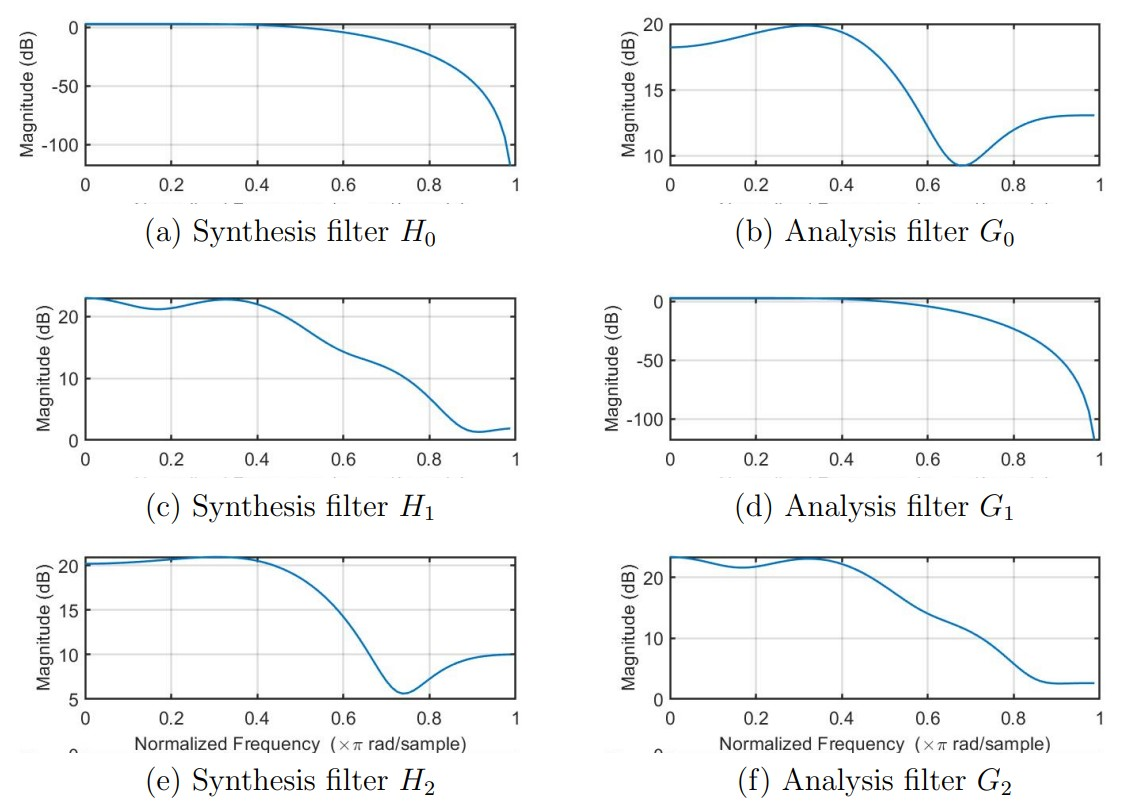
\includegraphics[width = 8.75cm]{mag_response_v2.jpg}
% \caption{Magnitude Response of the designed filters.}
% \label{mag}
% \end{figure}

\begin{figure*}[htpb]
\centering
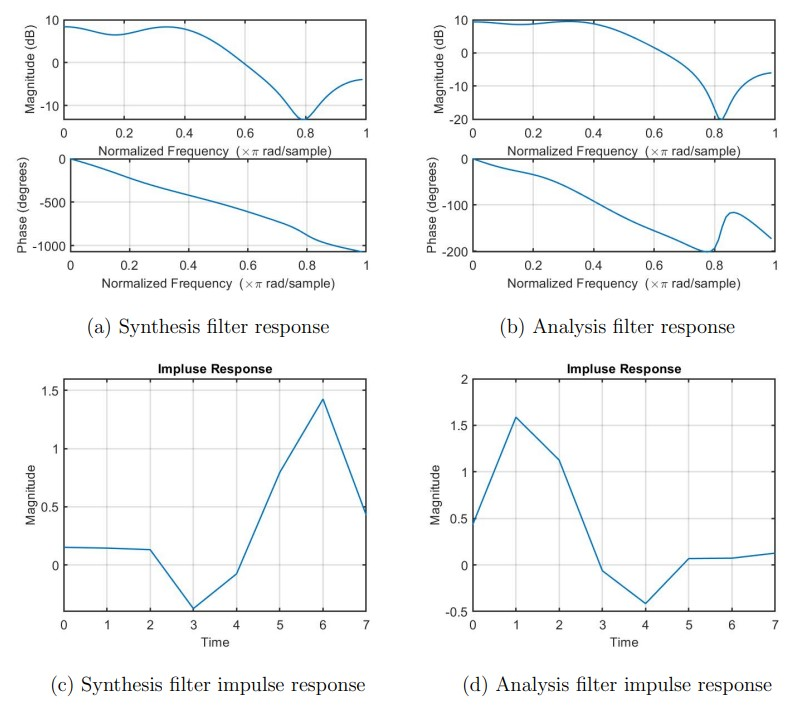
\includegraphics[width = 10.2cm]{agg_response_v2.jpg}
\caption{Aggregated response plots of the system.}
\label{agg}
\end{figure*}

Now that the filters are designed to meet the input signal specifications, they can be incorporated in the WT-based filter bank as a part of the trans-multiplexer system. The multiple signal inputs are then individually fed into the synthesis part of the system, where the filter bank performs the relevant processing. The processed signals are then added (concatenated) to be transmitted through the chosen channel model. In the receiver section, the received signal passes through the analysis part of the system, where the signals are perfectly reconstructed into their constituent parts. The output signals are then compared with the original input signals for error analysis and optimization of the system.

\subsection{Simulation using MATLAB}
This section describes the realization of the designed filters and the trans-multiplexer system as described above using MATLAB. The designed filter parameters are imported, and the input signals are defined. The WT-based DyadicAnalysisFilterBank and DyadicSynthesisFilterBank objects are then defined using the relevant designed filters \cite{b20}. These objects accept the ‘NumLevels’ parameter i.e. the frequency factor M = 4 for the selected case. The ‘Filter’ parameter can also be specified, which changes the wavelet family of the mother wavelet used to perform the transforms. The input signals are then passed through the DyadicSynthesisFilterBank object and are then added and transmitted over the channel model. The received signal is then passed through the DyadicAnalysisFilterBank object to reconstruct the original signals. A delay object is introduced in the system to model the transmission process effectively. The simulation uses MATLAB TimeScope objects to display the time-domain representation of the input, transmitted, reconstructed, and error signals. The simulation uses channel models (AWGN, Rician) to add noise to the transmitted signal and simulate real-world scenarios. A sine, square and saw-tooth signals with different frequencies and phase differences are used as test signals to simulate the performance of the implemented system. Fig. \ref{fig:input_signals} and \ref{fig:reconstructed_signals} show the time-domain waveform of the input and reconstructed signals respectively. From Fig. \ref{fig:input_spectrum} and \ref{fig:transmitted_spectrum}, we can see the effect of interpolation (x4) on the input signals by the synthesis filter bank. Fig. \ref{fig:transmitted_signal} shows the time-domain waveform of the transmitted signal.

\section{Results}
\subsection{Evaluation Metrics}
The simulation uses Mean Squared Error (MSE) of the normalized input and reconstructed signals to evaluate the implemented system. The MSE of the system is given by:

\begin{equation}
    MSE = \frac{1}{n}\sum_{i=1}^{n}(X_i-\hat{X}_i)^2
\end{equation}

where, \\
${n}$ = number of samples \\
$X_{i}$ = normalized input signal \\
$\hat{X}_{i}$ = normalized reconstructed signal

\subsection{Simulation Results}

\begin{figure}[htpb]
    \centering
    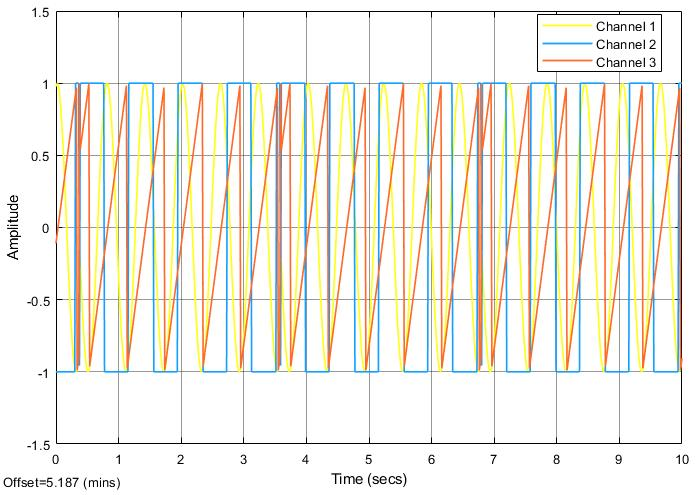
\includegraphics[width = 8.5cm]{original_signal.jpg}
    \caption{Time-domain waveform of input test signals.}
    \label{fig:input_signals}
\end{figure}

Table \ref{tab:sim} shows the MSE values of the system for various mother wavelets under different channel conditions for a Signal-to-noise ratio (SNR) of -20 dB (Without any channel, AWGN, and Rician). The Designed wavelet filter showcases an improvement of approximately 70 \% compared to other wavelet families. \par 

\begin{figure}
    \centering
    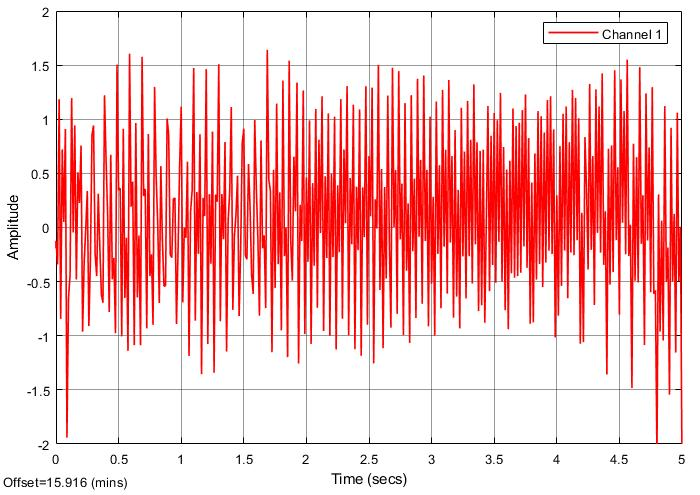
\includegraphics[width = 8.5cm]{transmitted_signal.jpg}
    \caption{Time-domain waveform of transmitted signal.}
    \label{fig:transmitted_signal}
\end{figure}

\begin{figure}
    \centering
    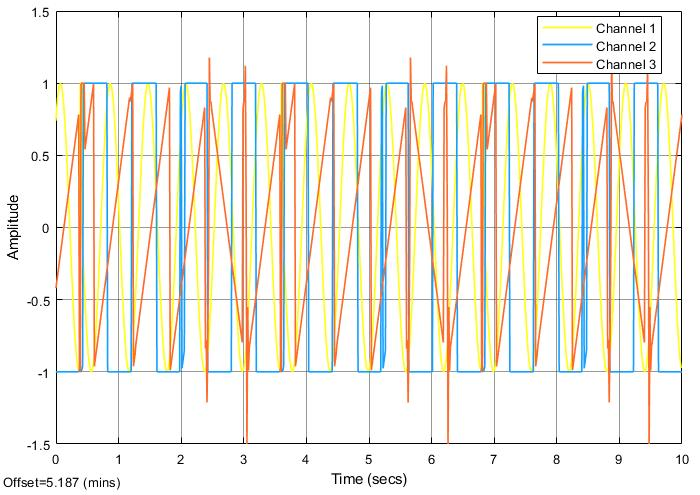
\includegraphics[width = 8.5cm]{reconstructed_signal.jpg}
    \caption{Time-domain waveform of reconstructed signals.}
    \label{fig:reconstructed_signals}
\end{figure}

\begin{figure}[htpb]
    \centering
    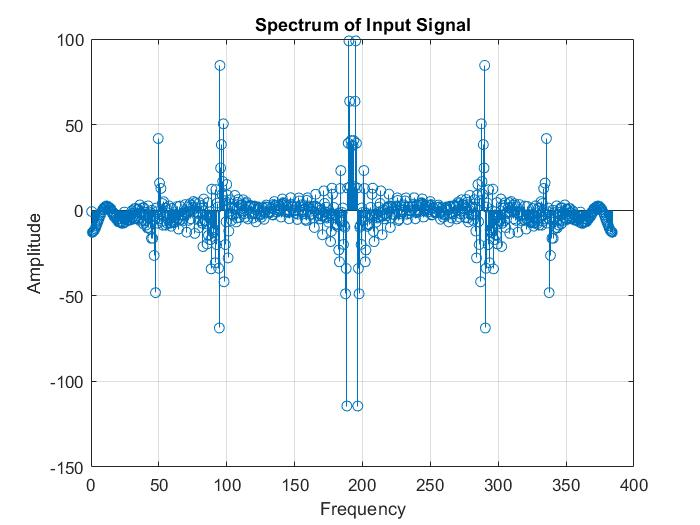
\includegraphics[width = 8.5cm]{Input_Spectrum.jpg}
    \caption{Spectrum of input test signals.}
    \label{fig:input_spectrum}
\end{figure}

\begin{figure}
    \centering
    \includegraphics[width = 8.5cm]{transmitted_Spectrum.jpg}
    \caption{Spectrum of transmitted signals.}
    \label{fig:transmitted_spectrum}
\end{figure}


\begin{table}[htpb]
  \centering
  \caption{\label{tab:sim}Mean Error Rate of the System for SNR = $-20 dB$}
  \resizebox{\columnwidth}{!}{%
  \begin{tabular}{|c|c|c|c|c|}
  \hline
    \multicolumn{4}{|c|}{Mean Error Rate} \\
    \hline
    & \multicolumn{3}{c|}{Channel Model} \\
    \hline
    Wavelet Family & No Channel & AWGN & Rician Fading \\
    \hline
    \multicolumn{1}{|c|}{Designed Filters} & 1.41 x $10^{-8}$ & 0.009215 & 0.0380 \\
    \hline
    \multicolumn{1}{|c|}{Haar} & 4.35 x $10^{-8}$ & 0.012177 & 0.0437   \\
    \hline
    \multicolumn{1}{|c|}{Daubechies} & 2.34 x $10^{-8}$ & 0.009020 & 0.0411 \\
    \hline
    \multicolumn{1}{|c|}{Symlets} & 2.75 x $10^{-8}$ & 0.010338 & 0.0484  \\
    \hline
    \multicolumn{1}{|c|}{Biorthogonal} & 3.16 x $10^{-8}$ & 0.013067 & 0.0455\\
    \hline
  \end{tabular}
  }
\end{table}

\begin{table}[htpb]
    \centering
    \caption{Mean Error Rate of the System for AWGN Channel.}
    \resizebox{\columnwidth}{!}{%
    \begin{tabular}{|c|c|c|}
    \hline
    \multicolumn{3}{|c|}{Mean Error Rate} \\
    \hline
       SNR (dB)  & Proposed system & Conventional system \\
       \hline
        -50 & 1.02 & 1.7982 \\
         \hline
         -30 & 0.042634 & 0.6528\\
         \hline
         -20 & 0.002215 & 0.1929\\
         \hline
         -5 & 0.000165 & 0.00807\\ 
         \hline 
         10 & 0.000023 & 0.00087\\ 
         \hline
         20 & 0.0000012 & 0.00042\\
         \hline 
         30 & 1.23 x $10^{-8}$ & 9.1590 x $10^{-5}$\\
         \hline
    \end{tabular}
    }
    \label{tab:error_awgn}
\end{table}

Table \ref{tab:error_awgn} shows the MSE values for the Proposed system that uses WT-based Filter banks for different SNR values through an AWGN channel. These values are compared with a corresponding Conventional system implemented using FT-based filter banks. The simulation is run for 100 times and the final mean error rate was calculated. The proposed system outperforms the conventional system by a factor of approximately $10^{-4}$. Fig. \ref{fig:error_plot_awgn} shows the MSE v/s SNR plot for the Proposed and Conventional system for an AWGN channel.


\subsection{Result Analysis}
This section discusses the results of the simulations obtained in this chapter. Table \ref{tab:sim} highlights that the designed wavelet filters improve upon the MSE by approximately 70 \% compared to other wavelets for various channel models. It performs especially well under Rician fading channel conditions that characterize interference under LoS conditions, a useful metric for satellite systems \cite{channel}. Generic wavelets are constructed using predefined equations, which do not work well with filter bank-based systems. The designed filters perform better as they are specially designed for trans-multiplexer systems and integrate well with the system requirements. 

\begin{figure}[htpb]
    \centering
    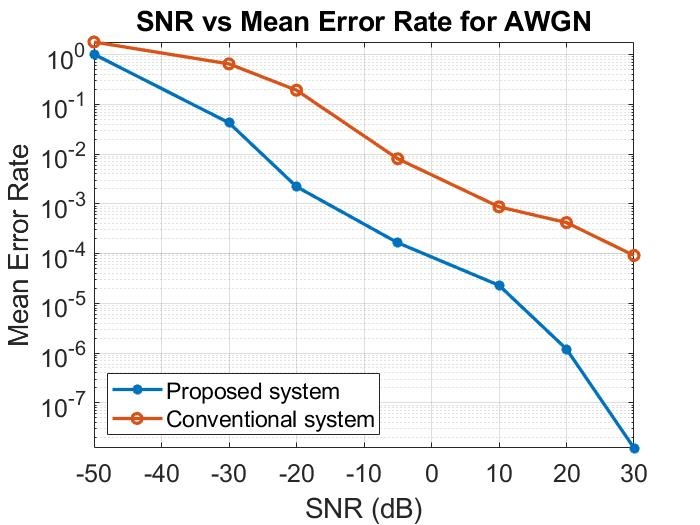
\includegraphics[width=8.75cm]{error_rate_awgn_v3.jpg}
    \caption{SNR v/s Mean Error Rate plot for AWGN Channel.}
    \label{fig:error_plot_awgn}
\end{figure}

Table \ref{tab:error_awgn} highlights the improvement in MSE for an AWGN channel achieved by the wavelet-based proposed system over the fourier-based conventional system. For low values of SNR, the performance of both systems is comparable. As the SNR values increase to about $-15$ dB, the proposed system outperforms the conventional system by a factor of approximately $10^{-4}$. The proposed system exhibits better performance as it uses DWT and is able to extract both temporal and frequency information from the signals, allowing better reconstruction. Table \ref{tab:time} highlights the improvement in time complexity achieved by the WT-based system. This is expected, as the time complexity of the WT-based system is $O(N)$ while that of FT-based system is $O(N*log(N))$.

\begin{table}[htpb]
    \centering
    \caption{Time Complexity of the Proposed and Conventional System.}
      \resizebox{\columnwidth}{!}{%
    \begin{tabular}{|c|c|c|}
    \hline
    System & Simulation Time & Processing Time \\
    \hline
         Proposed (WT) & 36.43 s  & 1.43 s\\
         \hline
         Conventional (FT) & 41.18 s & 6.18 s \\
         \hline
    \end{tabular}
    }
    \label{tab:time}
\end{table}

Hence, based on the result analysis, it is apparent that the designed 3-input WT-based system is objectively better than conventional FT-based systems, especially for satellite applications.

\subsection{Implementation using MATLAB HDL Coder}
This section explores the implementation of the designed system using the HDL Coder Toolbox in MATLAB. The HDL Coder facilitates the development, eumlation and verification of hardware designs and automatically generates synthesizable RTL code to target specific FPGAs. The HDL code generation for the system is done using 2 MATLAB functions for the transmitter and receiver, respectively. This allows the work to compare the software-based simulation to hardware-based implementations of the system. For the HDL Test Bench, the system uses two audio signals and one chip signal for simulation. For 15 dB of AWGN noise, the MSE of the simulated and emulated systems differed by 40.5 \%. Fig. \ref{fig:rtl} shows the RTL Schematic of the transmitter generated using the VHDL code from the Coder. 

\begin{figure*}[htpb]
    \centering
    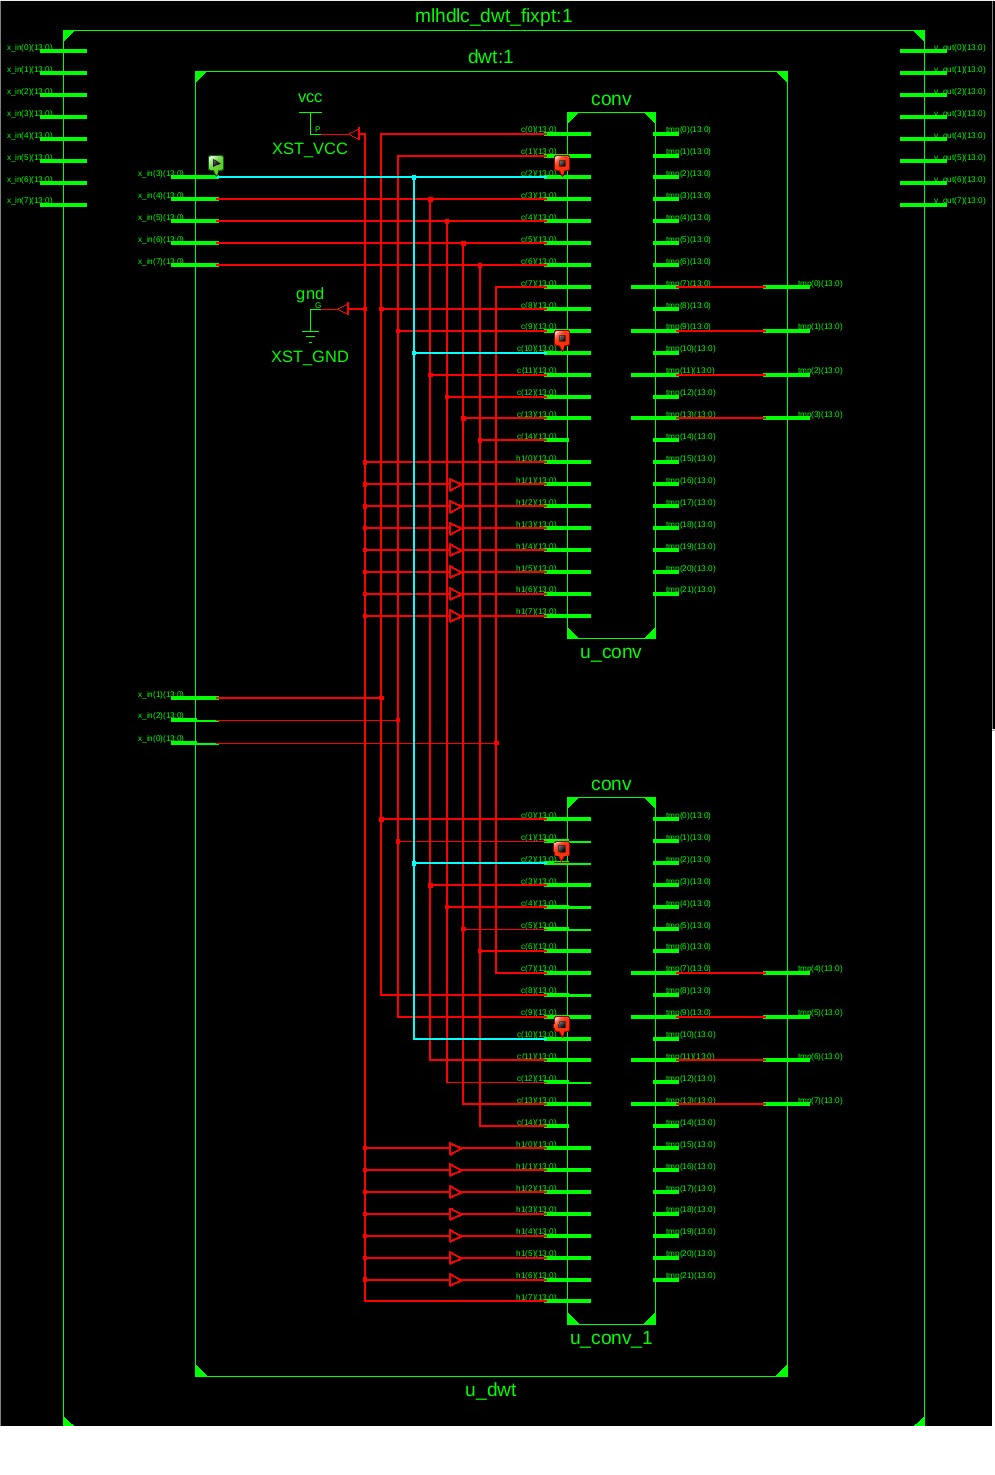
\includegraphics[width = 9.1cm]{rtl_schematic.png}
    \caption{RTL Schematic of the transmitter system.}
    \label{fig:rtl}
\end{figure*}

\section{Conclusion}
Multiplexing is an integral part of signal processing in satellite systems as it preserves channel resources while reducing the time and cost of signal transmission. The use of filter bank-based multiplexers will help improve the performance and reliability of satellite communication systems. trans-multiplexers are a widely explored application of Filter banks, which conventionally use Fourier-based filters to perform TDM-FDM conversion. This study proposes an algorithm to design wavelet transform-based filters for trans-multiplexer systems. The filters and the corresponding system are realized in MATLAB and are simulated under various conditions. The study evaluates the system using the Mean Squared Error (MSE) of the normalized signals. The work compares the performance of the designed wavelet filters with other wavelet families as well as a similar fourier-based conventional system. 

The proposed system improves upon the MSE of the conventional system by a factor of $10^{-4}$. The time complexity of the wavelet-based system is improved by a factor of $4.5$ which results in reduced signal processing time. Thus, it is apparent that the designed 3-input WT-based system is objectively better than conventional FT-based systems. The main limitation of the system is the poor reconstruction of signals with a high frequency of sharp fluctuations. Future studies can test the proposed algorithm by designing filters for different frequencies of operation. The trans-multiplexer system proposed in this paper can be implemented on an FPGA/ASIC to test its performance in real-world conditions.

\begin{thebibliography}{00}

% \bibitem{b0}
% M. O.  Oliveira, J. H.  Reversat, and L. A.  Reynoso, ``Wavelet Transform Analysis to Applications in Electric Power Systems'', in \textit{Wavelet Transform and Complexity}. London, United Kingdom: IntechOpen, 2019.

\bibitem{b1}
ISRO Research Proposals, 2021. \textit{ISRO Respond Basket.} [online] isro.gov.in., SAC-009 pg 44-45, Available at: https://www.isro.gov.in/sites/default/files/article-files/capacity-building/supported-areas-of-research/respond\_basket\_book-\_final-1.pdf, [Accessed 23 August 2021].

\bibitem{b2} 
Penedo, S.R.M., Netto, M.L. \& Justo, J.F. Designing digital filter banks using wavelets. \textit{EURASIP J. Adv. Signal Process. 2019}, 33 (2019). https://doi.org/10.1186/s13634-019-0632-6

\bibitem{b3}
Peter Yusuf Dibal, Elizabeth Onwuka, James Agajo, \& Caroline Alenoghena (2019). Analysis of Wavelet transform Design via Filter Bank Technique. In \textit{Wavelet transform and Complexity.} IntechOpen.

\bibitem{b5}
M. Vetterli and C. Herley, ``Wavelets and filter banks: theory and design,'' in \textit{IEEE transactions on Signal Processing}, vol. 40, no. 9, pp. 2207-2232, Sept. 1992, doi: 10.1109/78.157221.

\bibitem{b9}
M. Vetterli, ``Perfect transmultiplexers,'' ICASSP '86. IEEE International Conference on Acoustics, Speech, and Signal Processing, 1986, pp. 2567-2570, doi: 10.1109/ICASSP.1986.1169290.

\bibitem{b4}
C. Sidney Burrus, \textit{Wavelets and Wavelet transforms.} OpenStax CNX. Aug 6, 2018 http://cnx.org/contents/110bab92-1948-4958-b1c7-8fc0926c392c\@5.16. 

\bibitem{mallat_paper}
S. G. Mallat, ``A theory for multiresolution signal decomposition: the wavelet representation,'' in \textit{IEEE transactions on Pattern Analysis and Machine Intelligence}, vol. 11, no. 7, pp. 674-693, July 1989, doi: 10.1109/34.192463.

\bibitem{b16}
Akansu, A. N., Serdijn, W. A., \& Selesnick, I. W. (2010). Emerging applications of wavelets: A review. \textit{Physical Communication,} 3(1), 1-18. https://doi.org/10.1016/j.phycom.2009.07.001

\bibitem{b6}
Cruz-Roldan, F., Bravo-Santos, P, ``Design of multi-channel near-perfect-reconstruction transmultiplexers using cosine-modulated filter banks'', \textit{Elsevier Signal Processing} Volume 83 Issue, 5 May 2003, Pages 1079-1091

\bibitem{b10}
A. Vishwakarma, A. Kumar, \& G.K. Singh (2017). ``Design of near-perfect-reconstructed transmultiplexer using different modulation techniques: A comparative study''. Journal of King Saud University - Engineering Sciences, 29(3), 257-263.

\bibitem{b7}
Ramachandran, R., \& Kabal, P. (1990). ``transmultiplexers: Perfect reconstruction and compensation of channel distortion''. \textit{Signal Processing}, 21, 261-274.

\bibitem{b8}
Martin Vetterli (1986). ``Filter banks allowing perfect reconstruction''. \textit{Signal Processing}, 10(3), 219-244.

\bibitem{b14}
M. Vetterli, ``A theory of multirate filter banks,'' in \textit{IEEE transactions on Acoustics, Speech, and Signal Processing}, vol. 35, no. 3, pp. 356-372, March 1987, doi: 10.1109/TASSP.1987.1165137.

\bibitem{b13}
Ting Liu, \& Tongwen Chen (2000), ``Optimal design of multi-channel transmultiplexers''. \textit{Elsevier Journal on Signal Processing}, 80(10), 2141-2149.

\bibitem{b11}
Ali Naci Akansu, Richard A. Haddad, and Hakan Caglar ``Perfect reconstruction binomial QMF-wavelet transform'', Proc. SPIE 1360, \textit{Visual Communications and Image Processing '90:} Fifth in a Series, (1 September 1990); https://doi.org/10.1117/12.24246

\bibitem{b15}
N. Mishra, P. Mishra, H. Shah and A. Banik, ``A design method using a set of objective functions for near-perfect reconstruction filter bank based transmultiplexer for onboard transparent processor,'' \textit{2013 International Conference on Signal Processing and Communication (ICSC)}, 2013, pp. 271-275, doi: 10.1109/ICSPCom.2013.6719796.

\bibitem{b20}
MathWorks. 2021. Three-Channel Wavelet transmultiplexer. [online] Available at: <https://in.mathworks.com/help/dsp/ug/three-channel-wavelet-transmultiplexer.html> [Accessed 6 October 2021].

\bibitem{channel} Lu Lu, Daoxing Guo, Aijun Liu, \& Maoqiang Yang (2012), ``Analysis of Channel Model for GEO Satellite Mobile Communication System'', In Proceedings of the \textit{2012 National Conference on Information Technology and Computer Science} (pp. 863-867). Atlantis Press.

\end{thebibliography}
\end{document}
